\section{Methods and Materials}
\label{sec:methods}

In Fall of 2020\footnote{The work described here was originally planned for Spring 2020 but has been shifted due to the global COVID-19 pandemic.}, I plan to use the RoboRoach kit (Backyard Brains; Ann Arbor, MI) kit to apply electrical stimulation to a cockroach's antenna, causing it to turn in the contralateral direction when I apply current. The kit includes a printed circuit board (PCB), which is a backpack that carriers the Bluetooth Low Energy wireless receiver/transmitter, which will allow communication between my smartphone and the backpack. It also includes a battery for the backpack and three electrode sets for three cockroaches, each of which include one electrode for each antenna and one for ground, since electricity needs a closed circuit and the electrical stimulation current needs a return pathway. The kit also consists of all the items necessary for surgery\footnote{Fine forceps (tweezers), forceps (hemostat), a loupe, a low temperature hot glue gun, hot glue sticks, Q-tips, sandpaper, loctite super glue, a popsicle stick, silly putty, dissection scissors, flour, a needle, and toothpicks. In addition to the kit, I will need a cup of ice water, paper towels, a clock, and a work lamp.}. As a first step, I will use the Backyard Brains surgery protocols to prepare neuro-implanted RoboRoaches. Based on what I learn in the first iterations, I may adapt the surgery protocols as necessary. 





\subsection{Experimental subjects}
Experiments will be conducted with two species of cockroach that are readily available through the pet trade. I will order at least five adult \emph{Periplaneta americana} (American cockroaches). I will also use three adults of either \emph{Blaberus discoidalis} (discoid cockroach) or \emph{Gromphadorhina portentosa} (Madagascar hissing cockroaches). Animals will be kept in separate terrariums, bedded with wood chips, and provided with food (Purina Puppy Chow) and water \emph{ad libitum}. As methods are tested, I would ideally scale up to have at least 10 healthy adult cockroaches to test on. 




\subsection{Surgery}
I will follow the general surgical protocols from \citep{backyardbrains2020roboroach}. Surgery will be conducted on one cockroach at a time. Animals will be anesthetized by submergence in ice water for \SIrange{2}{5}{\minute}, until they fail to respond to mechanical stimuli. The electrode array is then attached to the pronotum, a connector is added, and insect pins and cyanoacrylate adhesive are used to implant the ground and sensing electrodes. Finally, wires are attached and strain relieved. The detailed protocol for electrode implantation surgery is given in appendix~\ref{app:A}. 








\subsection{Open loop checks of electrode function}
After recovery from surgery, I will test electrode function using the RoboRoach app \citep{backyardbrains2020roboroach}. To test stimulation of the antennae, I will plug the male connector of the PCB into the female connector on the roach's head. Using the app, I will apply the default stimulation settings and swipe left or right to observe behavioral responses. The surgery is successful if the cockroach turns in the direction I swiped. In addition, I will evaluate open loop performance by steering the cockroach open loop and measuring the angle of turn upon stimulation, using either machine vision tracking or an arena marked in \ang{30} increments. For each experiment, I would either film cockroach kinematics from above, or use a timer to measure the time it took for a cockroach to react to the stimulation and the electrical tape to measure the angle of turn. 






\subsection{Plant estimation and closed loop control experiments}
With the cockroaches that successfully turn left and right when stimulated, I will place them on track made of thin strips of electrical tape consisting of straight paths and \ang{90} turns and observe their ability to make it all the way through. I will also test the roach's ability to turn to various angles by modulating the current sent to its antennae and evaluating its performance of different maneuvers such as the Dieudonne Spiral, a siunsoid, and a zig-zag. My hope is that these maneuvers would provide data to attempt some kind of plant estimation and would lead to eventual closed-loop roach-in-the-loop testing with an offboard sensor (notionally, a camera) and controller. \Fref{fig:rough} displays the open and closed loop diagrams for the experiment, as well as sketches of maneuvers that can be performed to evaluate directional control.
\begin{figure}[ht!]
\begin{center}
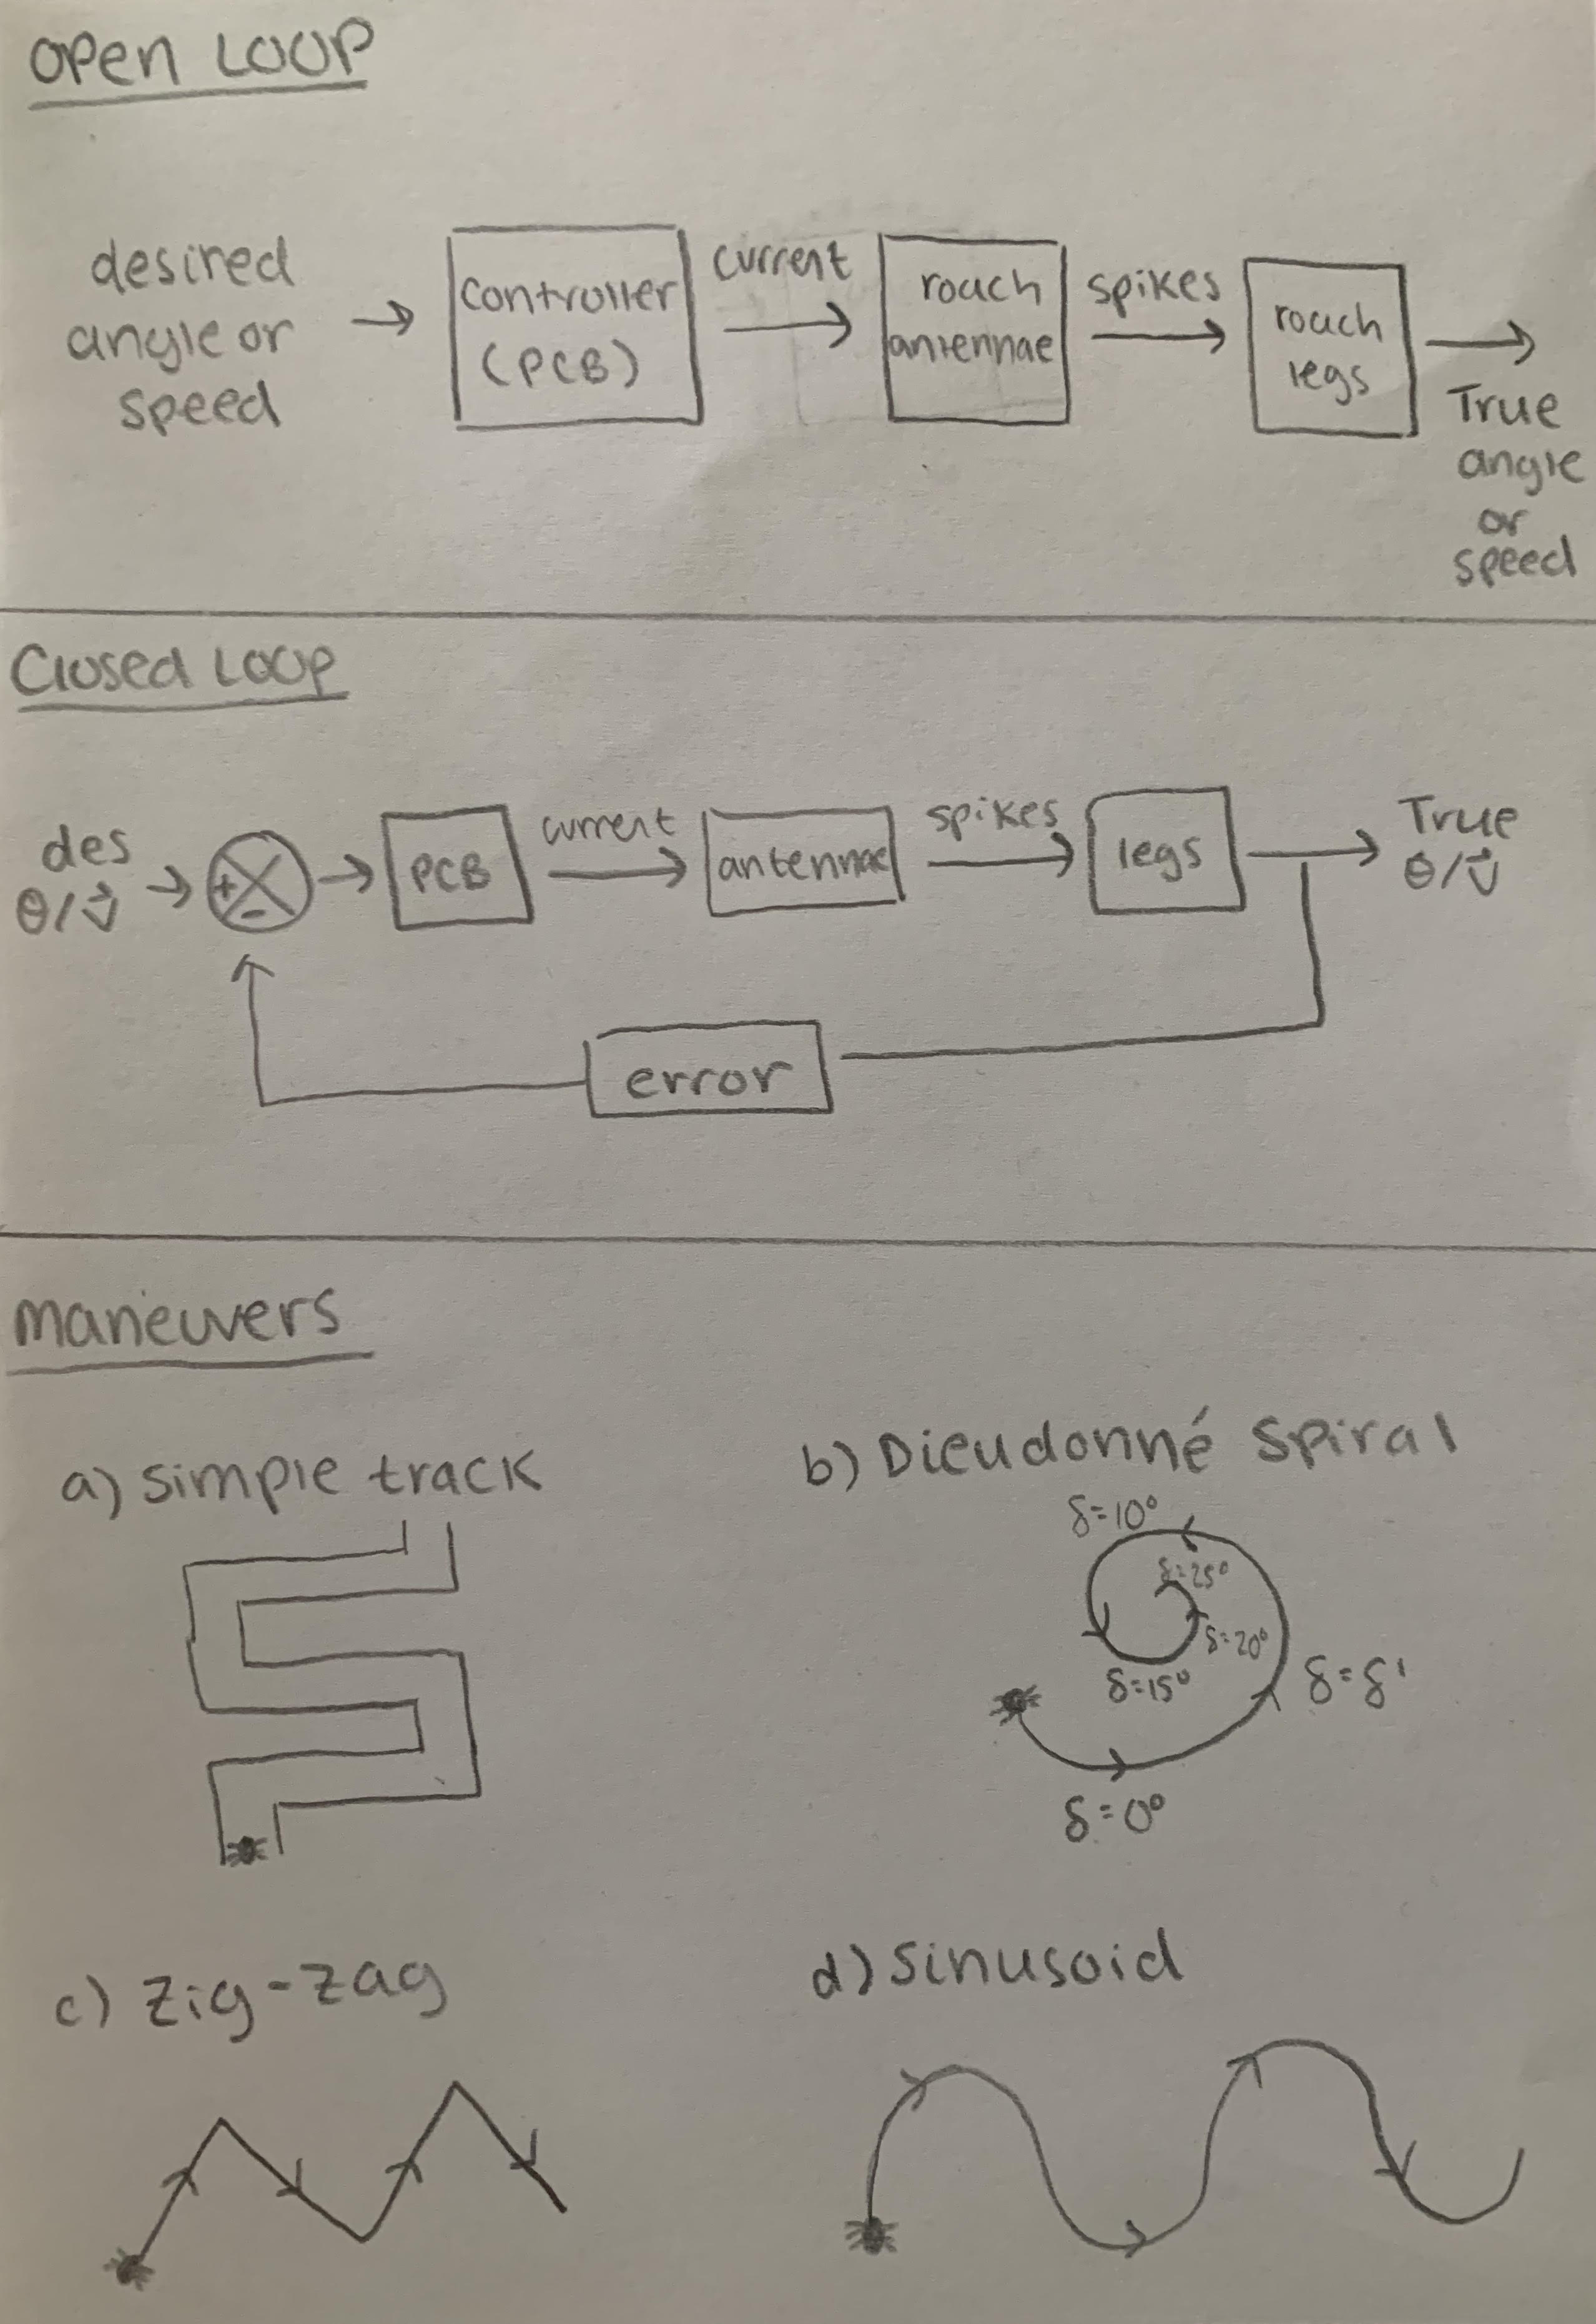
\includegraphics[scale=0.1]{Figures/olcl.jpg}
\end{center}
\caption{Notional open- and close-loop diagrams and maneuevers to be attempted with RoboRoach.}
\label{fig:rough}
\end{figure}

Assuming that I could control forward motion and the sharpness of the turn by modulating the current sent to the roach's antenna, I could evaluate performance through various maneuvers. For a counterclockwise Dieudonne Spiral, a maneuver used to examine stability and turning performance in ships. I would start by having the roach move forward in one direction. Then I would gently stimuate its right antenna, turning the roach to the left in slight increments of about \ang{5} every \SI{2}{\second} to achieve the large outer portion of the spiral. Once it has almost made a complete circle, I would stimulate its right antenna at a higher level, turning the roach in increments of about \ang{15} to achieve a smaller spiral. Then I would stimulate its right antenna at an even higher level, turning the roach in increments of about \ang{30} to achieve the smallest inner spiral.

In addition, closed loop control is often probed using steps, ramps, and sinusoids.  For the sinusoid, I would execute a similar pattern of stimulation as the Dieudonne Sprial, but I would need to stimulate both antennae. I would start by having the roach move forward in one direction. Then I would stimuate its left antenna, turning the roach to the right by about \ang{10}. I would let the roach continue on the path until its position was nearly at my desired peak. Once the roach started to approach the peak of the sinusoid, I would stimulate its left antenna multiple times to achieve multiple right turns of about \ang{30} until it was on a downward path. I would let the roach continue on the downward path until its position was nearly at my valley. Once the roach started to approach the valley of the sinusoid, I would stimulate its right antenna multiple times to achieve multiple left turns of about \ang{30} until it was on an upward path again.

For the zig-zag, I would start by having the roach move forward in one direction. Then I would sharply stimuate its right antenna, turning the roach to the left by about \ang{90}. After letting the roach move forward in its new direction for about \SI{5}{\second}, I would sharply stimulate its left antenna, turning the roach to the right by about \ang{90}, letting it walk in its new direction for about \SI{5}{\second} before having it turn again.

Once directional control is achieved, I will try to achieve speed control. Stimulation to the antennae may not necessarily control speed in addition to direction, so I will attempt to stimulate other areas of the roach's body to change its speed.  For example, the cerci on roaches are wind sensors at the posterior end that elicit full ahead escape running.  



























